% !TEX program = XeLaTeX
% !TEX encoding = UTF-8
\documentclass[UTF8]{ctexart}
%{ctexart}


%\setCJKmainfont[BoldFont=FandolSong-Bold.otf,ItalicFont=FandolKai-Regular.otf]{FandolSong-Regular.otf}
%\setCJKsansfont[BoldFont=FandolHei-Bold.otf]{FandolHei-Regular.otf}
%\setCJKmonofont{FandolFang-Regular.otf}

\usepackage{url}
\usepackage{cancel}
\usepackage{xspace}
\usepackage{graphicx}
\usepackage{multicol}
\usepackage{multirow}
\usepackage{subfig}
\usepackage{amsmath}
\usepackage{amssymb}
%\usepackage[a4paper, width=186mm, top=18mm, bottom=18mm, includeheadfoot]{geometry}
\usepackage[a4paper, width=140mm, top=18mm, bottom=22mm, includeheadfoot]{geometry}
\usepackage{booktabs}
\usepackage{array}
\usepackage{verbatim}
\usepackage{caption}
\usepackage{natbib}
\usepackage{booktabs}
\usepackage{float}
\usepackage{pdflscape}
\usepackage{mathtools}
\usepackage[usenames, dvipsnames]{xcolor}
\usepackage{afterpage}
\usepackage{pgf}
\usepackage{tikz}
\usepackage{dirtree}
\usepackage{amsmath}
\usepackage{pst-plot,pst-eucl}
\usepackage[nomessages]{fp}
\usepackage[style=american]{csquotes}
\usepackage{amsfonts}
\usepackage{tikz}
\usepackage{tkz-graph}
\usetikzlibrary{arrows,decorations.pathmorphing,automata,positioning,backgrounds,fit,shapes.symbols,chains,intersections}

\pagecolor[rgb]{0.18,0.18,0.18}

\newtheorem{definition}{定义}[section]
\newtheorem{theorem}{Theorem}[section]
\newtheorem{lemma}{Lemma}
\newtheorem{proof}{Proof} [section]

\usepackage[toc, page, title, titletoc, header]{appendix}
\usepackage{marginnote}
\usepackage{tablefootnote}

\renewcommand\appendixname{附\ 录}
\renewcommand\appendixpagename{附\ 录}
\renewcommand\appendixtocname{附\ 录}
\renewcommand\abstractname{摘要}


\usepackage{perpage} %the perpage package
\MakePerPage{footnote} %the perpage package command

\usetikzlibrary{shapes.geometric}%
\usepackage{color}
%\usepackage[pages=some, placement=top]{background}
\usepackage{eso-pic}
\usepackage[final]{pdfpages}

%\includepdf[pages=1]{cover}
\hyphenpenalty=750
\AtBeginDocument{\color{white}}
\title{\textbf{Oedax: 一种开放式的荷兰拍卖交易模式}}
\author{
  王东\\
  \texttt{daniel@loopring.org}\\
%  \and
%  	郭雄辉\\
%  	\texttt{steve@loopring.org}
 }

\makeatletter
\def\CTEX@section@format{\Large\bfseries}
\makeatother

\makeatletter
\newenvironment{tablehere}
 {\def\@captype{table}}
 {}

\newenvironment{figurehere}
 {\def\@captype{figure}}
 {}
\makeatother
%
%\newcommand\BackgroundPic{%
%\put(0, 0){%
%\parbox[b][\paperheight]{\paperwidth}{%
%\vfill
%\centering
%\includegraphics[width=\paperwidth, height=\paperheight, %
%%keepaspectratio]{images/background.jpg}%
%]{images/background.jpg}%
%\vfill
%}}}


\begin{document}
%\AddToShipoutPicture{\BackgroundPic}
\maketitle


\begin{abstract}
我们通过这篇文章介绍一种基于荷兰式拍卖的新型数值货币交易模式: Open-Ended Dutch Auction eXchange,简称Oedax。相对于基于原始荷兰式拍卖的交易模式,如DutchX,Oedax可能具有交易者更喜欢的一些新特性。
\end{abstract}


\section{荷兰式拍卖}

荷兰式拍卖又称为减价拍卖。在拍卖过程中,商品价格不断降低,直到有足够多的购买者将商品全部买走。所有买家最终付的成交价都一样,无论在竞拍过程中出价是多少。

\begin{center}
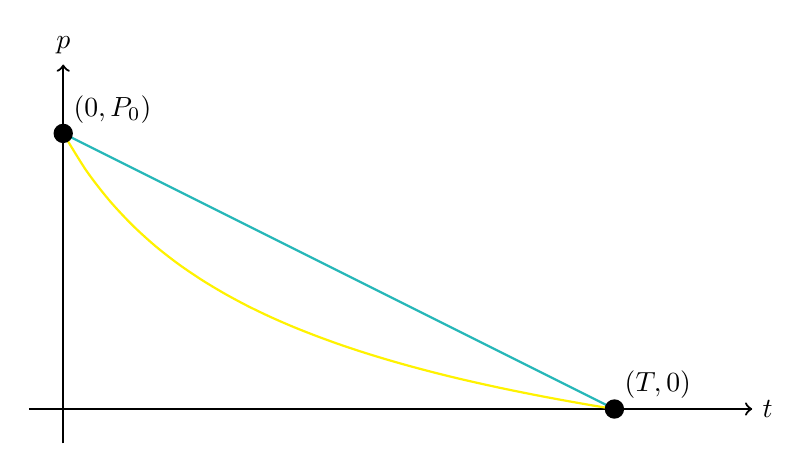
\begin{tikzpicture}[thick, scale=1.75]
      \draw[->] (-0.25,0) -- (5,0) node[right] {$t$};
      \draw[->] (0,-0.25) -- (0,2.5) node[above] {$p$};
      \draw[scale=1,domain=0:4,smooth,variable=\x,yellow] plot ({\x},{2*(1/sqrt(\x+1)- 1/sqrt(5))/(1-1/sqrt(5))});
      \draw[scale=1,domain=0:4,smooth,variable=\x, BlueGreen] plot ({\x},{(2-\x/2)});
%      \node [fill, draw, circle, minimum width=3pt, inner sep=0pt, pin={[fill=white, outer sep=2pt]135:P}] at (.5,1) {$abc$};
%      \draw plot[mark=*, only marks] coordinates {((4,0)};
%      
      \fill (0,2)  circle[radius=2pt] node[above right] {$(0,P_0)$};
      \fill (4,0)  circle[radius=2pt] node[above right] {$(T,0)$};                    
    \end{tikzpicture}
\end{center}

\bibliography{oedax_whitepaper}
\bibliographystyle{unsrt}


%\end{multicols}


%\begin{appendices}
%
%
%\end{appendices}
\end{document}
